\problemname{Tile Traveller}

The assignment is to develop a computer game in which a player is located in a grid of tiles,
one of which is occupied by the player.
At each iteration, the program displays the directions
for which there are adjacent tiles that the player can travel to.

The program only displays text, so you do not actually draw the tile grid,
but the program should behave as if the player is in a $3 \times 3$ grid,
as seen in the following image:

\begin{figure}[h]
    \centering
    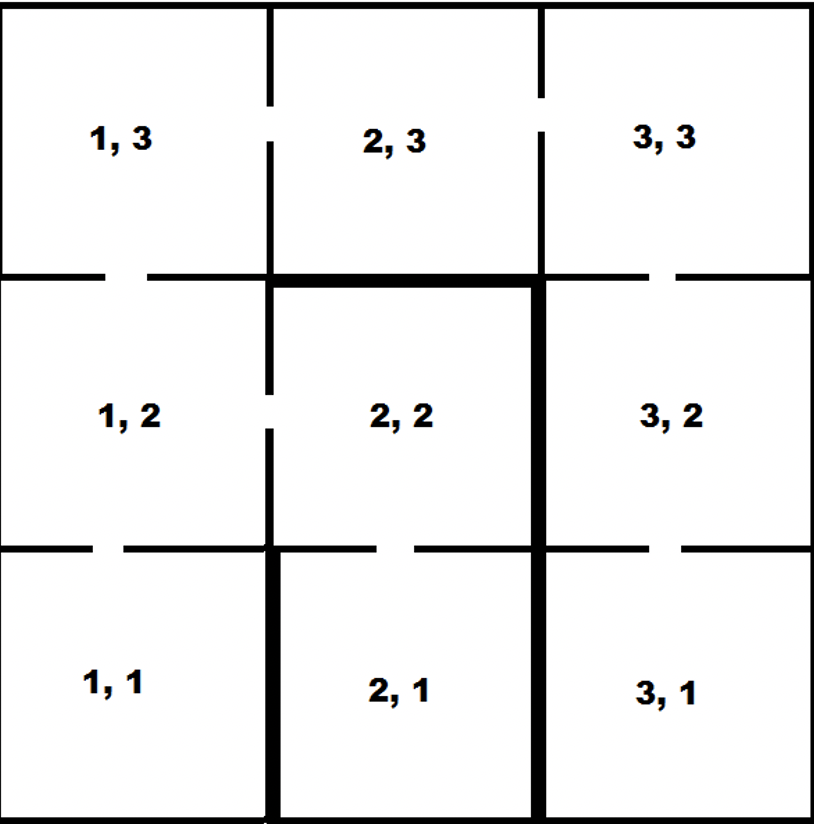
\includegraphics[width=0.33\textwidth]{maze}
    \caption{\texttt{Maze}}
\end{figure}

As indicated in the image, there are walls between some adjacent tiles,
blocking the player from travelling directly between them.
In other cases, there's an open path from one tile to the next.
You may think of these open paths as doorways, or just the absence of walls,
it does not matter, the effect is the same.

The player starts in tile \texttt{(1, 1)}.
At the beginning, and after each move selected by the player,
the program should print the player's travel options.
If there is no wall in a given direction,
write that direction as a possible travel direction.

At each iteration, the player enters the first letter of the direction in which they wish to travel,
after which the player should be located in another tile and the options for the new tile are then printed out.

The order in which the directions should be listed, is \emph{North, East, South, West}.

The player enters:
\begin{itemize}
    \item n/N for North (up)
    \item e/E for East (right)
    \item s/S for South (down)
    \item w/W for West (left)
\end{itemize}

If the player enters an invalid direction,
the program prints ``\texttt{Not a valid direction!}''
and prompts the player to enter the direction again.

For example, in tile \texttt{(1,1)} it is only possible to move north.
In tile \texttt{(1,2)} the possible moves are north, east, and south.
In tile \texttt{(3,3)} the possible moves are south and west.

Tile \texttt{(3,1)} is the victory location.
When the player enters this tile, the program should notify them of their victory and quit.

\section*{Input}
Input consists of one line for each move made by the player, in order,
where each move consists of any of the characters
\texttt{n}, \texttt{e}, \texttt{s}, \texttt{w}, \texttt{N}, \texttt{E}, \texttt{S}, or \texttt{W}.
These lines repeat until the player has won the game.
It is guaranteed that the player will win the game in less than $200$ moves.

\section*{Output}

First, the program should print ``\texttt{You can travel: \{Valid directions\}.}'',
without quotations, where valid directions can be
\texttt{(N)orth}, \texttt{(E)ast}, \texttt{(S)outh}, and \texttt{(W)est}.
The directions should be separated by spaces and the word ``\texttt{or}''.
The following repeats until the user wins the game,
at which point the program exits after outputting a victory message:
\begin{itemize}

    \item The program prompts the user with ``\texttt{Direction: }'', without quotations.
    \item If the player inputs an invalid direction, the program should output ``\texttt{Not a valid direction!}'', without quotations.
    \item If the player inputs a valid direction, the program should output the new valid directions as stated above, 
        ``\texttt{You can travel: \{Valid directions\}.}'', without quotations.
    \item If the player wins, the program should output ``\texttt{Victory!}'', without quotations.

\end{itemize}
